% Copyright (C) 2010,2011,2012,2013,2014,2015,2016 The ESPResSo project
% Copyright (C) 2002,2003,2004,2005,2006,2007,2008,2009,2010 
%   Max-Planck-Institute for Polymer Research, Theory Group
%  
% This file is part of ESPResSo.
%   
% ESPResSo is free software: you can redistribute it and/or modify it
% under the terms of the GNU General Public License as published by the
% Free Software Foundation, either version 3 of the License, or (at your
% option) any later version.
%  
% ESPResSo is distributed in the hope that it will be useful, but
% WITHOUT ANY WARRANTY; without even the implied warranty of
% MERCHANTABILITY or FITNESS FOR A PARTICULAR PURPOSE.  See the GNU
% General Public License for more details.
%  
% You should have received a copy of the GNU General Public License
% along with this program.  If not, see <http://www.gnu.org/licenses/>.
%
%%%%%%%%%%%%%%%%%%%%%%%%%%%%%%%%%%%%%%%%%%%%%%%%%%%%%%%%%%%%%%%%% 
% From the brainstorming:
%
% Preknowledge:
% 
% Basic MD(simple integrator,langevin thermostat, ---basic tcl
% basic potentials, basis tutorial 1
% 
% Basis Tutorial: written in Latex
% 
% <<every line of script code should be explained>>
% 
% 1) tcl basic setting up a system
% MD, soft sphere and Lennard-Jones Fluid (argon system), 
% Units
% 
% online visualization (pdb output)
% rdf, pressure,energy,
% 
% online analysis function
% savin, readin writeout, offline analysis, statistics
% 
% Structure:
% Part1:
% 1) Prerequisits (what you should know beforehand: basic tcl knowledge,
% Here you can find more info: Allen, Tildesley: Frenkel smit,
% Rappaport, tcl tutorial,
% 
% 2) Physics of the systems (argon, soft sphere system)
% 
% 3) Algorithms (verlocity verlet, Langevin, Potentials, LJ)
% 3b) about units
% 
% Part2 
% 1) simulation script in all detail, line by line
% Initialize
% Visualize
% Simulate (with online analysis, saves for later off-line analysis,
% (Savelize (save our lives ))
% 
% 2) a new script for later
% analysis, and other helper ideas
% 
% Things to remember and take care of:
% Use the same names for variables
% 
% ====================================================================
% General Tutorial: (the next tutorials: pe_solution, cell model of one
% charged colloid, LB, ferrofluid)
% 
\documentclass[
paper=a4,                       % paper size
fontsize=11pt,                  % font size
twoside,                        % two sided
footsepline,                    % add a line to separate the footer
headsepline,                    % add a line to separate the header
headinclude=false,              % header does not belong to the text
footinclude=false,              % footer does not belong to the text
pagesize,                       % set the pagesize in a DVI document
]{scrartcl}

% Copyright (C) 2010,2011,2012 The ESPResSo project
% Copyright (C) 2002,2003,2004,2005,2006,2007,2008,2009,2010
%  Max-Planck-Institute for Polymer Research, Theory Group
%  
% This file is part of ESPResSo.
%   
% ESPResSo is free software: you can redistribute it and/or modify it
% under the terms of the GNU General Public License as published by the
% Free Software Foundation, either version 3 of the License, or (at your
% option) any later version.
%  
% ESPResSo is distributed in the hope that it will be useful, but
% WITHOUT ANY WARRANTY; without even the implied warranty of
% MERCHANTABILITY or FITNESS FOR A PARTICULAR PURPOSE.  See the GNU
% General Public License for more details.
%  
% You should have received a copy of the GNU General Public License
% along with this program.  If not, see <http://www.gnu.org/licenses/>.
%
\usepackage[draft]{varioref}    % defines \vref
\usepackage{hyperref}           % automatically creates links when
                                % using pdflatex, defines \url
\usepackage{ifpdf}              % defines \ifpdf
\usepackage{graphicx}           % handles graphics
\usepackage{color}              % use colors

\usepackage{amsmath}

\usepackage{verbatim}           % required for \verbatim and \endverbatim
\usepackage{fancyvrb}
\usepackage{calc}               % compute length
\usepackage{ifthen}             % provide ifthen
\usepackage{xspace}
\usepackage{units}
\usepackage[numbers]{natbib}

% For building the distribution docs, disable todo boxes.
%\usepackage[disable]{todonotes}
\usepackage{todonotes}

\newcommand{\es}{\mbox{\textsf{ESPResSo}}\xspace}
\newcommand{\ie}{\textit{i.e.}\xspace}
\newcommand{\eg}{\textit{e.g.}\xspace}
\newcommand{\etal}{\textit{et al.}\xspace}

\newcommand{\codebox}[1]%
{\texttt{#1}}

\DefineVerbatimEnvironment{code}{Verbatim}%
{commandchars=\\\{\}}
\makeatletter
\newenvironment{tclcode}
{%
  \addtolength{\linewidth}{-2em}% set the line length
  \@minipagetrue%%%DPC%%%
  \@tempswatrue%%%DPC%%%
  \hsize=\linewidth%
  \setbox0=\vbox\bgroup\verbatim
}{\endverbatim
  \unskip\setbox0=\lastbox%%%DPC%%%
  \egroup
  \par%
  \noindent\hspace{1em}%
  \codebox{\box0}%
  \par\noindent%
}
\makeatother

% \newcommand{\todo}[1]{
%   \marginpar{%
%     \setlength{\fboxrule}{1pt}
%     \fcolorbox{red}{yellow}{%
%       \parbox{\marginparwidth-2\fboxrule-2\fboxsep}{%
%         \bf\raggedright\scriptsize #1%
%       }%
%     }%
%   }%
% }

\makeatletter
\renewcommand{\minisec}[1]{\@afterindentfalse \vskip 1.5ex
  {\parindent \z@
    \raggedsection\normalfont\sffamily\itshape\nobreak#1\par\nobreak}%
  \@afterheading}
\makeatother

\newcommand{\esptitlehead}{
  \titlehead{
    \begin{center}
      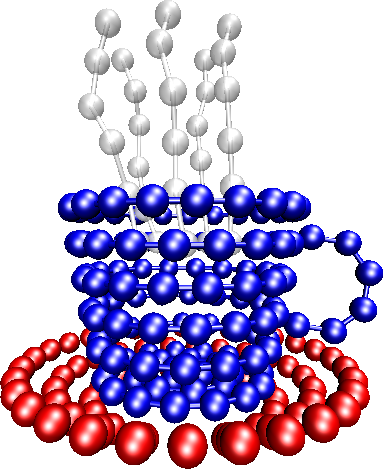
\includegraphics[width=5cm]{logo/transparentbg}
    \end{center}
  }
}


%% Grafikpakete
\usepackage{graphicx}%


\usepackage{verbatim}

% How to diplay ESPResSo commands in flowing text. Larger code segments
% should be put inside boxes.
\newcommand{\EScmd}[1]{\texttt{\textbf{#1}}}

% The code block
%\newcommand{\EScode}[1]{ \parbox{0.95\textwidth}{\texttt{#1}}}
\usepackage{listings} 
\lstset{numbers=left, numberstyle=\tiny, numbersep=5pt, showspaces=false, showstringspaces=false,postbreak=\space, breakindent=5pt, breaklines}
\lstset{language=python, keywordstyle=\color{blue}\bfseries ,emphstyle=\color{green}, commentstyle=\color{red}\itshape }
\lstset{keywordsprefix=setmd}
\lstset{keywords=[6]{thermostat,part,inter,integrate,rescale_velocities,code_info,save_sim,writepdb,analyze,uwerr}}

\newtheorem{task}{Task}

% Copyright (C) 2010,2011,2012 The ESPResSo project
% Copyright (C) 2002,2003,2004,2005,2006,2007,2008,2009,2010
%  Max-Planck-Institute for Polymer Research, Theory Group
%  
% This file is part of ESPResSo.
%   
% ESPResSo is free software: you can redistribute it and/or modify it
% under the terms of the GNU General Public License as published by the
% Free Software Foundation, either version 3 of the License, or (at your
% option) any later version.
%  
% ESPResSo is distributed in the hope that it will be useful, but
% WITHOUT ANY WARRANTY; without even the implied warranty of
% MERCHANTABILITY or FITNESS FOR A PARTICULAR PURPOSE.  See the GNU
% General Public License for more details.
%  
% You should have received a copy of the GNU General Public License
% along with this program.  If not, see <http://www.gnu.org/licenses/>.
%
\usepackage[draft]{varioref}    % defines \vref
\usepackage{hyperref}           % automatically creates links when
                                % using pdflatex, defines \url
\usepackage{ifpdf}              % defines \ifpdf
\usepackage{graphicx}           % handles graphics
\usepackage{color}              % use colors

\usepackage{amsmath}

\usepackage{verbatim}           % required for \verbatim and \endverbatim
\usepackage{fancyvrb}
\usepackage{calc}               % compute length
\usepackage{ifthen}             % provide ifthen
\usepackage{xspace}
\usepackage{units}
\usepackage[numbers]{natbib}

% For building the distribution docs, disable todo boxes.
%\usepackage[disable]{todonotes}
\usepackage{todonotes}

\newcommand{\es}{\mbox{\textsf{ESPResSo}}\xspace}
\newcommand{\ie}{\textit{i.e.}\xspace}
\newcommand{\eg}{\textit{e.g.}\xspace}
\newcommand{\etal}{\textit{et al.}\xspace}

\newcommand{\codebox}[1]%
{\texttt{#1}}

\DefineVerbatimEnvironment{code}{Verbatim}%
{commandchars=\\\{\}}
\makeatletter
\newenvironment{tclcode}
{%
  \addtolength{\linewidth}{-2em}% set the line length
  \@minipagetrue%%%DPC%%%
  \@tempswatrue%%%DPC%%%
  \hsize=\linewidth%
  \setbox0=\vbox\bgroup\verbatim
}{\endverbatim
  \unskip\setbox0=\lastbox%%%DPC%%%
  \egroup
  \par%
  \noindent\hspace{1em}%
  \codebox{\box0}%
  \par\noindent%
}
\makeatother

% \newcommand{\todo}[1]{
%   \marginpar{%
%     \setlength{\fboxrule}{1pt}
%     \fcolorbox{red}{yellow}{%
%       \parbox{\marginparwidth-2\fboxrule-2\fboxsep}{%
%         \bf\raggedright\scriptsize #1%
%       }%
%     }%
%   }%
% }

\makeatletter
\renewcommand{\minisec}[1]{\@afterindentfalse \vskip 1.5ex
  {\parindent \z@
    \raggedsection\normalfont\sffamily\itshape\nobreak#1\par\nobreak}%
  \@afterheading}
\makeatother

\newcommand{\esptitlehead}{
  \titlehead{
    \begin{center}
      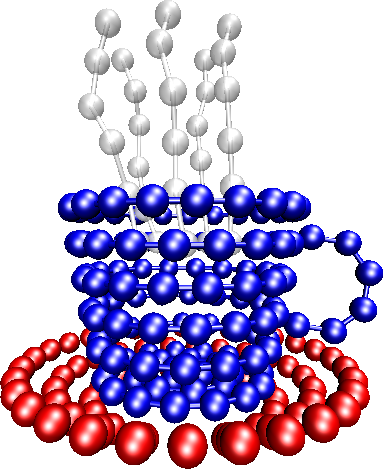
\includegraphics[width=5cm]{logo/transparentbg}
    \end{center}
  }
}


\begin{document}

\esptitlehead

\title{Tutorial 1: Lennard-Jones Liquid%
\ifdefined\esversion%
\thanks{For \es \esversion}%
\fi%
}
\subtitle{\es Basics}
\author{H.-J. Limbach \and M. S\"uzen \and K. Grass \and M. Sega \and
  A. Arnold \and N. Gribova}
\maketitle
\tableofcontents

\section{Introduction}

Welcome to the basic \es{} tutorial!

In this tutorial, you will learn, how to use the \es{} package for your 
research. We will cover the basics of \es, i.e., how to set up and modify a 
physical system, how to run a simulation, and how to load, save and analyze
the produced simulation data.

More advanced features and algorithms available in the \es{} package are 
described in additional tutorials.


\section{Background}

Today's research on Soft Condensed Matter has brought the needs for having a 
flexible, extensible, reliable, and efficient (parallel) molecular simulation 
package. For this reason \es{} (Extensible Simulation Package for Research on 
Soft matter) \cite{esp_url} has been developed at Max Planck Institute for 
Polymer Research, Mainz, and Institute for Computational Physics at the University of Stuttgart in  the group of Prof. Dr. Christian Holm\cite{limbach2006ees,arnold13a}. The Espresso package is probably the most flexible and 
extensible simulation package in the market. It is specially developed for 
coarse-grained molecular dynamics (MD) simulation of polyelectrolytes but not 
necessarily limited to this. It can be used even in simulating granular media 
for example. \es{} has been nominated for the Heinz-Billing-Preis for 
Scientific Computing in 2003 \cite{arnold2003ees}.

\subsection{The Lennard-Jones Potential}

A pair of neutral atoms or molecules is subject to two distinct forces in the limit
of large separation and small separation: an attractive force at long ranges (van der
Waals force, or dispersion force) and a repulsive force at short ranges (the result
of overlapping electron orbitals, referred to as Pauli repulsion from Pauli exclusion
principle). The Lennard-Jones potential (also referred to as the L-J potential, 6-12
potential or, less commonly, 12-6 potential) is a simple mathematical model that
represents this behavior. It was proposed in 1924 by John Lennard-Jones. The L-J
potential is of the form
\begin{math}
\label{eq:lj}
    V(r) = 4\epsilon [{({\frac{\sigma}{r}})}^{12} - (\frac{\sigma}{r})^{6}]
\end{math}
where $\epsilon$ is the depth of the potential well and $\sigma$ is the (finite)
distance at which the inter particle potential is zero and $r$ is the distance between
the particles. The $(\frac{1}{r})^{12}$ term describes repulsion and the
$(\frac{1}{r})^{6}$  term describes attraction. The Lennard-Jones potential is an
approximation. The form of the repulsion term has no theoretical justification; the
repulsion force should depend exponentially on the distance, but the repulsion term
of the L-J formula is more convenient due to the ease and efficiency of computing
$r^{12}$ as the square of $r^6$.

\subsection{Units}

Novice users must understand that Espresso has no fixed unit system. The unit 
system is set by the user. Conventionally, reduced units are employed, in other 
words LJ units.
\footnote{If we have charges there is additionally a concept of Bjerrum length, consult Espresso original paper for more details.} 

\section{First Steps}\label{sec:espresso}

What is \es{}? It is not a coffee, indeed. It is an extensible, efficient 
Molecular Dynamics package specially powerful on simulating charged systems. 
In depth information about the package can be found in the relevant sources\cite{esp_url,arnold2003ees,limbach2006ees,arnold13a}.

\es consists of two components.
The simulation engine is written in C and C++ for the sake
of computational efficiency. The steering or control
level is interfaced to the kernel via an interpreter 
of the Python scripting languages.

The kernel performs all computationally demanding tasks. Before all,
integration of Newton's equations of motion, including calculation of
energies and forces. It also takes care of internal organization of
data, storing the data about particles, communication between
different processors or cells of the cell-system. 

The scripting interface (Python) is used to setup the system (particles, boundary conditions,
interactions, \dots), control the simulation, run analysis, and store and load results.
The user has at hand the full reliability and functionality of the scripting language.
For instance, it is possible to use the SciPy package for analysis and PyPlot for plotting.
With a certain overhead in efficiency, it can also be
used to reject/accept new configurations in combined MD/MC schemes. In
principle, any parameter which is accessible from the scripting level can be
changed at any moment of runtime. In this way methods like
thermodynamic integration become readily accessible.

\emph{Note: This tutorial assumes that you already have a working \es{}
installation on your system. If this is not the case, please consult the first
chapters of the user's guide for installation instructions.}


Using the pypresso script in the build directory, python simulation scripts can be run conveniently:

\vspace{0,2cm}
\noindent\texttt{./pypresso simulation.py}

\vspace{1cm}\framebox{
    \begin{minipage}{0.95\textwidth} 
        \begin{task} 
             You can check the features, that are compiled in the \es{} core by
             issuing \texttt{print(code\_info.features())} after having imported the 
             \texttt{code\_info} Module:
        \end{task}
    \end{minipage}
}\vspace{1cm}

\begin{pypresso}
from espressomd import code_info
print(code_info.features())
\end{pypresso}


\section{Overview over a Simulation Script}

Typically, a simulation script consists of the following parts
\begin{itemize}
\item System setup (box geometry, thermodynamic ensemble, integrator parameters)
\item Placing the particles
\item Setup of interactions between particles
\item Warmup (bringing the system into a state suitable for measurements)
\item Integration loop (propagate the system in time and record measurements)
\end{itemize}
In the following sections, it will be shown, how these steps can be taken. Once the basics are covered, we apply them to the simulation of the Lennard-Jones liquid.
Note, that only the core elements of the Lennard-Jones simulation script will be covered in this document. The full script can be found in the under \verb+scripts/lj_tutorial.py+ in the Lennard-Jones tutorial directory.


\subsection{System Setup}
The functionality of \es{} for
python is provided via a python module called
\texttt{espressomd}. At the beginning of the simulation script, it has to be imported.
\begin{pypresso}
import espressomd
\end{pypresso}

The next step would be to create an instance of the System class. 
This instance is used as a handle to the simulation system. It can be used to manipulate the
crucial system parameters like the time step and the size of the simulation box (\texttt{time\_step}, and \texttt{box\_l}). At any time, only one instance of the System class can exist.
\begin{pypresso}
system = espressomd.System()
system.time_step = time_step
system.box_l = [box_l_x, box_l_y, box_l_z]
\end{pypresso}
\subsection{Choosing the thermodynamic ensemble, thermostat}
Simulations can be carried out in different thermodynamic ensembles such as NVE (particle
Number, Velocity, Energy) or NVT (particle Number, Velocity, Temperature)
as well as NPT-isotropic (particle Number, Pressure, Temperature). 
The ensemble is maintained by a thermostat. In this tutorial we use the Langevin thermostat.

In \es{}, the thermostat is set as follows:
{\small\vspace{0,2cm}
\begin{pypresso}
system.thermostat.set_langevin(kT=1.0, gamma=0.5)
\end{pypresso}}\vspace{0,2cm}
\noindent Use a Langevin thermostat (NVT ensemble) with temperature set to 1.0 and damping coefficient to 0.5. Alternatively, the thermostat can be turned off using
{\small\vspace{0,2cm}
\begin{pypresso}
system.thermostat.turn_off()
\end{pypresso}}\vspace{0,2cm}
\noindent This results in an NVE ensemble.


\subsection{Placing and Accessing Particles}

Particles in the simulation can be accessed via the \texttt{part}-property of the System class. Individual particles are referred to by an integer id, e.g., \texttt{system.part[0]}. It is also possible to use common python iterators and slicing operations to access several particles at once.
\begin{pypresso}
# access position of single particle
print system.part[0].pos

# Iterate over particles
for p in system.part:
    print(p.pos)
    print(p.v)

#Obtain all particle positions
cur_pos = system.part[:].pos
\end{pypresso}
Particles can be grouped into several types, so that, e.g., a binary fluid can be simulated. Particle types are identified by integer ids, which are set via the particles' \texttt{type} attribute. 

Particles are added to the simulation as follows
\begin{pypresso}
system.part.add(id=0, type=0, pos=[x,y,z])
\end{pypresso}\vspace{0,2cm}
Here, \texttt{id} and \texttt{type} can be omitted, in which case an unused particle
id is assigned automatically and type 0 is implied.

Many objects in \es{} have a string representation, and thus can be displayed via python's \texttt{print} method:
\begin{pypresso}
print system.part[0]
\end{pypresso}\vspace{0,2cm}


\subsection{Setting up Non-Bonded Interactions}

Non-bonded interactions act between all particles of a given combination of particle types.
In this tutorial, we use the Lennard-Jones non-bonded interaction.
The interaction of two particles of type 0 can be setup as follows:
{\small\vspace{0,2cm}
\begin{pypresso}
lj1_eps     = 1.0
lj1_sig     = 1.0
lj1_cut     = 1.12246
lj1_shift   = 0.0
lj1_offset  = 0.0
system.non_bonded_inter[0, 0].lennard_jones.set_params(epsilon=lj_eps, sigma=lj_sig,
cutoff=lj_cut, shift=lj_shift)
\end{pypresso}
}\vspace{0,2cm}


\subsection{Warmup}

In many cases, including this tutorial, particles are initially placed randomly in the simulation box. It is therefore possible that particles overlap, resulting in a huge repulsive force between them. In this case, integrating the equations of motion would not be numerically stable. Hence, it is necessary to remove this overlap.
This is done by limiting the maximum force between two particles, integrating the equations of motion, and increasing the force limit step by step.
This is done as follows
\begin{pypresso}
# Obtain minimum distance between particles
act_min_dist = system.analysis.mindist()
lj_cap=10
while i < warm_n_time and act_min_dist < lj_sigma*0.9 :
    # Set the force cap
    system.non_bonded_inter.set_force_cap(lj_cap)
    lj_cap += 1.0
    # Integrate the equation of motion
    system.integrator.run(100)
    # Obtain minimum distance between particles
    act_min_dist = system.analysis.mindist()

# Disable force cap
system.non_bonded_inter.set_force_cap(0)
\end{pypresso}
In this code fragment, you can also see, how the analysis routines can be used to obtain information about the simulation system, and how to integrate the equation of motion.


\section{Putting It All Together: Lennard-Jones Liquid Simulation}

After we have briefly explained the use of \es{}, we now come to the
Lennard-Jones Liquid Simulation.  Before we explain the script step by step, run the
\texttt{lj\_tutorial.py}  with \texttt{pypresso} to get all generated files.


\subsection{Initialization}

First, we include necessary modules with \lstinline|import|.
{\small\vspace{0,2cm}
\begin{pypresso}
import espressomd

from __future__ import print_function
import cPickle as pickle
import os 
import numpy as np

print("""
=======================================================
=                    lj_tutorial.py                   =
=======================================================

Program Information:""")
print(code_info.features())
\end{pypresso}\vspace{0,2cm}

\subsubsection{System Setup}
At first, we must configure the environment and set the needed parameters.
It is good practice to define all simulation parameters as variables in a single location.
{\small\vspace{0,2cm}
\begin{pypresso}
# System parameters
#############################################################
# Number of particles and density
n_part  = 108
density = 0.8442

skin        = 0.1
time_step   = 0.001 
eq_tstep    = 0.0001
temperature = 0.728

box_l       = np.power(n_part/density, 1.0/3.0) + 2*skin

warm_steps  = 100
warm_n_time = 2000
min_dist    = 0.87

# Integration
sampling_interval       = 10
equilibration_interval  = 1000

sampling_iterations     = 10000
equilibration_iterations= 20

# Interaction parameters (Lennard-Jones)
#############################################################

lj_eps = 1.0
lj_sig = 1.0
lj_cut = 2.5
lj_cap = 20

# System setup
#############################################################
system              = espressomd.System()

if not os.path.exists('data') :
    os.mkdir('data')

system.time_step    = time_step
system.cell_system.skin  = skin

system.box_l = [box_l, box_l, box_l]

system.non_bonded_inter[0, 0].lennard_jones.set_params(
    epsilon=lj_eps, sigma=lj_sig,
    cutoff=lj_cut, shift="auto")
system.non_bonded_inter.set_force_cap(lj_cap)

print("LJ-parameters:")
print(system.non_bonded_inter[0, 0].lennard_jones.get_params())

# Thermostat
system.thermostat.set_langevin(kT=temperature, gamma=1.0)
\end{pypresso}


\subsection{Particles}

\begin{pypresso}
# Particle setup
#############################################################

volume = box_l * box_l * box_l

for i in range(n_part):
    system.part.add(id=i, pos=np.random.random(3) * system.box_l)
\end{pypresso}}\vspace{0,2cm}

   \vspace{1cm}\framebox{\begin{minipage}{0.95\textwidth} 
   \begin{task}    
   Study the file \texttt{lj\_tutorial.py}. This system mimics the case 
   study 4 of section 4, in the book \cite{frenkel02b}. How can one define 
   truncated-shifted potential in \texttt{lj\_tutorial.py}? ( keep in mind 
   that Espresso has already a factor of 4 at shifted part with cut off 
   $r_{c}=2.5$)
    \[ U(r)= 4 \epsilon\left[ \left(\frac{\sigma}{r} \right)^{12} -  \left(\frac{\sigma}{r} \right)^{6} \right] \]
     
     \[ U(r)^{\text{tr-sh}}  =\left\{ \begin{array}{ll}  U(r)-U(r_{c})  &  r_{c} > r \\
     
     0 &   r_{c}  < r \end{array} \right. \]
     
  (To find the solution look at line 26. Look at picture \ref{pic:lennard-jones} to see a plot of the potential )

   \end{task}

\end{minipage}}\vspace{1cm}

\begin{figure}[ht]
\begin{center}
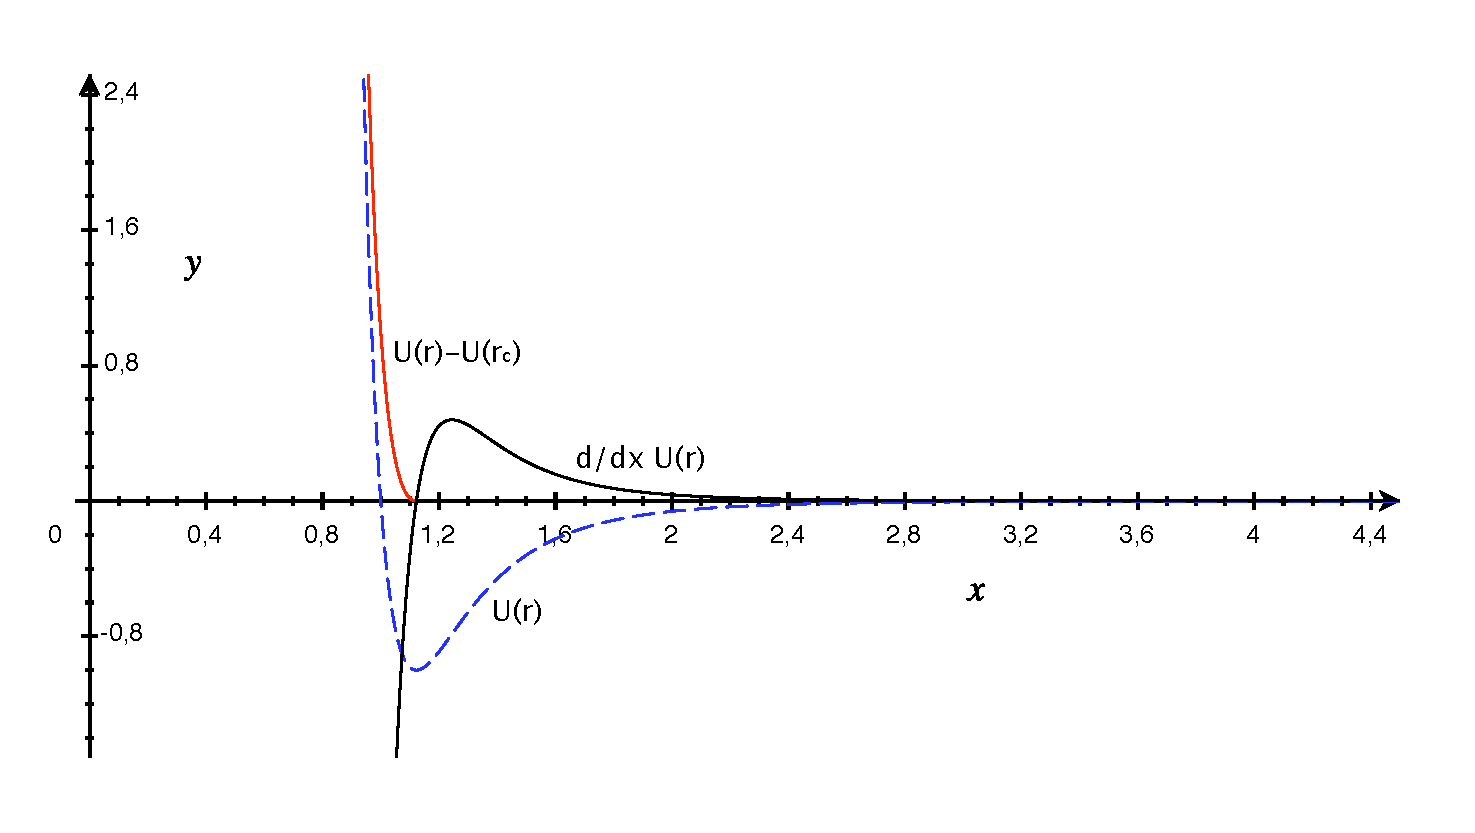
\includegraphics[width=12cm]{figures/lennard-jones-potential.pdf}
%\caption{Lennard Jones Potential - \newline ttt}
\caption[long text]{Lennard-Jones Potential with
  $\epsilon=1$ and radius $\sigma=1$. If you use a large cutoff such as
  $2.5\sigma$, the potential is practically zero at the cutoff. The
  red curve indicates the Weeks-Chandler-Andersen potential, which
  is obtained from the Lennard-Jones potential by cutting it off in
  its minimum at $r_c=\sqrt[6]{2}$ and shifting it up.}
\label{pic:lennard-jones}
\end{center}
\end{figure}


%\subsection{Warmup}
%
%After we have set the necessary environment we must warmup our system before we run the simulation. We set particles at random positions, so some particles can overlap. In this situation \es  will crash with an error:
%particle out of range. To remove the overlap between particles, we cap forces  by setting the Lennard-Jones force constant below a certain distance. 
%This is done using the \lstinline|set_force_cap| command. We do the procedure  \verb"warm_n_times" times 
%for \verb"warm_steps" steps and stop only if the minimal distance between particles is also larger than 
%\verb"min_dist", which was set earlier.  To turn 
%the capping off, we set \verb|set_force_cap(0)|. Then we equilibrate our system
%until all relevant physical observables are fluctuating around their mean values. In
%the case of Lennard-Jones it is enough to monitor energy.  To equilibrate we use the
%Langevin thermostat set to the target temperature.
%
%
%{\small\vspace{0,2cm}
%\begin{pypresso}
%#############################################################
%#  Warmup Integration                                       #
%#############################################################
%
%print("""
%Start warmup integration:
%At maximum {} times {} steps
%Stop if minimal distance is larger than {}
%""".strip().format(warm_n_time, warm_steps, min_dist))
%
%i = 0
%act_min_dist = system.analysis.mindist()
%while i < warm_n_time and act_min_dist < min_dist :
%    system.integrator.run(warm_steps)
%    act_min_dist = system.analysis.mindist()
%    print("run {} at time = {} (LJ cap= {} ) min dist = {}".strip().format(i, system.time, lj_cap, act_min_dist))
%    i+=1
%    lj_cap += 1.0
%    system.non_bonded_inter.set_force_cap(lj_cap)
%
%system.non_bonded_inter.set_force_cap(0)
%
%print("\nWarm up finished\n")
%
%system.time_step = eq_tstep 
%
%for i in range(equilibration_iterations):
%    system.integrator.run(equilibration_interval)
%    energies = system.analysis.energy()
%    print("eq run {} at time {}\n".format(i, system.time))
%
%print("\nEquilibration done\n")
%# Switch thermostat off NVE msd measurement
%system.thermostat.turn_off()
%
%\end{pypresso}}\vspace{0,2cm}

\subsection{Integrating the Equations of Motion, Taking Measurements}
\noindent At this point, we have set the necessary environment and warmed up our system. As a last
step before starting the actual simulation, we now open the files which we want to output data to
during the simulation. Then the simulation is started.

\begin{pypresso}
print("\nSampling\n")
system.time_step = time_step

en_fp   = open('data/energy.dat', 'w')
sys_fp  = open('data/sim_info.pickle', 'w')
part_fp = open('data/part.pickle', 'w')
msd_fp  = open('data/msd.dat', 'w')
rdf_fp  = open('data/rdf.dat', 'w')

en_fp.write("#\n#\n#\n# Pressure   Kinetic Potential   Temperature\n#\n")

# start positions of all particles for MSD calculation on the fly
start_pos=system.part[:].pos

# save system setup
pickle.dump(system, sys_fp, -1)
pickle.dump(system.part, conf_fp, -1)

msd = np.zeros((sampling_iterations,))

# save start particle configuration
pickle.dump(system.part, part_fp, -1)

for i in range(1, sampling_iterations + 1):
    system.integrator.run(sampling_interval)
    energies = system.analysis.energy()
    pressure = system.analysis.pressure()

    kinetic_temperature = energies['ideal']/( 1.5 * n_part)

    en_fp.write("%i\t%1.5e\t%1.5e\t%1.5e\t%1.5e\t%1.5e\n" % (i, pressure['total'], energies['total'], energies['ideal'], energies['total'] - energies['ideal'], kinetic_temperature))
\end{pypresso}}\vspace{0,2cm}

In the energy.dat file we print out the values for pressure, kinetic
and potential energies, temperature obtained with the analysis submodule
\lstinline|system.analysis.energy()|. See the code in the snippet above, which
contains the main sampling loop of the script.

\noindent \texttt{kinetic temperature} here refers to the measured temperature
obtained from kinetic energy and the number of degrees of freedom in the system. It
should fluctuate around the preset temperature of the thermostat.

\newpage
\vspace{1cm}\framebox{\begin{minipage}{0.95\textwidth} 
    \begin{task}
      Plot the time evolution of pressure and energy, which are written into the
      \texttt{data} directory in the file \texttt{energy.dat}.
    \end{task}
  \end{minipage}}\vspace{1cm}

The result plot for \texttt{energy.dat}
should be similar to this one:
\begin{center}
  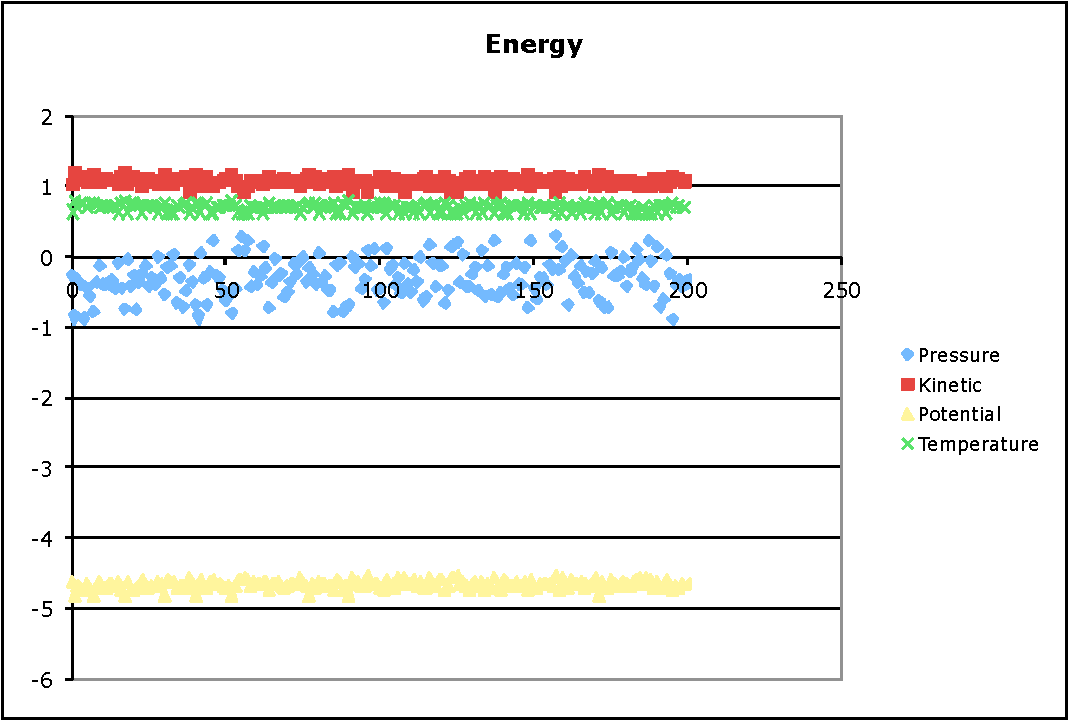
\includegraphics[width=10cm]{figures/energy}
\end{center}
\noindent As we can see the system is in equilibrium because pressure, potential, and kinetic energy per particle 
and calculated current temperature fluctuate around their mean values.

%%%%%%%%%%%%%%%%%%%%%%%%%%%%%%%%%%%%%%%%%%%%%%%%%%%  
   
% TODO:
% Once uwerr is available in Python a more elaborate error analysis will be possible
\subsection{Simple Error Estimation on Time Series Data}
A simple way to estimate the error of an observable is to use the common standard
deviation ($\sqrt{\sigma}$) and the standard error of the mean (SE) for $N$
\emph{uncorrelated} samples:
\begin{align}
    \sigma  &= \langle x^2 - \langle x\rangle^2 \rangle \\
    SE      &= \sqrt{\frac{\sigma}{N}}
    \label{eq:variance}
\end{align}

\begin{pypresso}
# Data arrays for simple error estimation
etotal = np.zeros((sampling_iterations,))
ptotal = np.zeros((sampling_iterations,))
for i in range(1, sampling_iterations + 1):
    energies = system.analysis.energy()
    pressure = system.analysis.pressure()

    etotal[i-1] = energies['total']
    ptotal[i-1] = pressure['total']

# calculate the variance of the total energy and total pressure using scipys statistic operations
error_total_energy=np.sqrt(etotal.var())/np.sqrt(sampling_iterations)
error_total_pressure=np.sqrt(ptotal.var())/np.sqrt(sampling_iterations)

en_fp.write("#mean_energy energy_error mean_pressure pressure_error\n#%1.5e %1.5e %1.5e %1.5e" % \
\end{pypresso}

\newpage


\subsection{Online Analysis of Correlations}

\label{subsection:online_analysis}
% TODO 
% Once the correlator found its way into the python interface this section has to be
% written 

This section will be updated once the correlator functionality is available in the
python interface.


\subsection{Other Useful Scripts}

\label{subsection:other_useful_scripts}
The radial distribution function (rdf) describes the distribution of particles around
the center of a fixed particle, as a function of the particle-particle distance. This of course assumes
that the particle distribution is isotropic around the particles.

The rdf is computed on the fly in the current script, the data is then written to
\texttt{data/rdf.dat}.

In order to compute the rdf with \texttt{espressomd} one needs the following code
fragments:
\begin{pypresso}
# analyzing the radial distribution function
# setting the parameters for the rdf
r_bins = 30
r_min  = 0.0
r_max  = system.box_l[0]/2.0

avg_rdf=np.zeros((r_bins,))

# calculate the rdf in the main sampling loop
for i in range(1, sampling_iterations + 1):
    system.integrator.run(sampling_interval)
    r, rdf = system.analysis.rdf(rdf_type="rdf", type_list_a=[0], type_list_b=[0], r_min=r_min, r_max=r_max, r_bins=r_bins)
    # system.analysis.rdf() return the bin positions as numpy array, here 'r'
    # and the corresponding value of the radial distribution function also as
    # numpy array in 'rdf'

    avg_rdf+= rdf/sampling_iterations
    # simply averaging over the calculated rdf and saving it to the ``average'' rdf
    # 'avg_rdf'
    

# after the sampling is done write out the radial distribution data and then close
# the file
for i in range(r_bins):
    rdf_fp.write("%1.5e %1.5e\n" % (r[i], avg_rdf[i]))

rdf_fp.close()
\end{pypresso}

\begin{figure}[ht]
\begin{center}
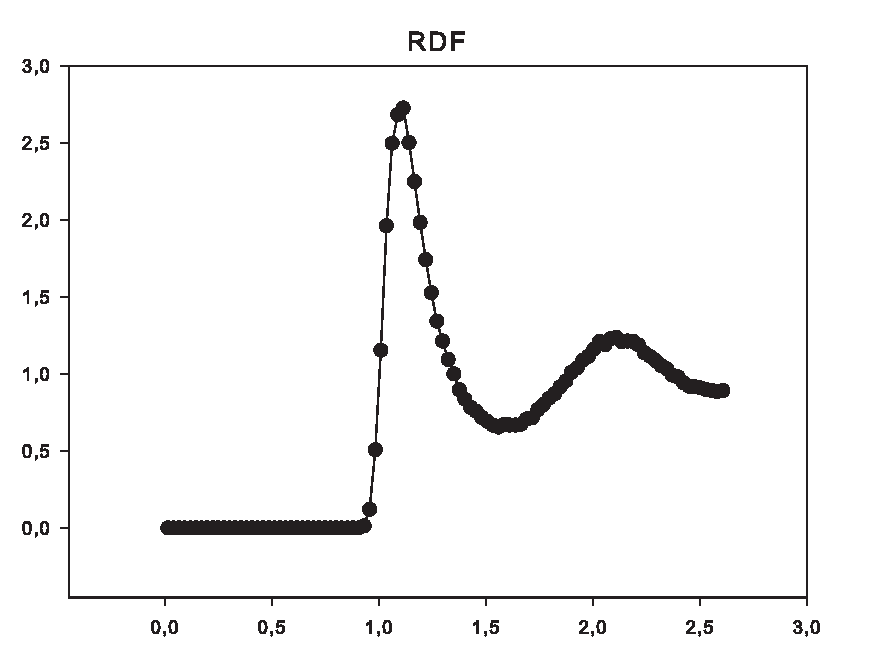
\includegraphics[width=10cm]{figures/rdf}
\label{fig:rdf}
\caption{The rdf.dat plot should be similar to this one}
\end{center}
\end{figure}


\section{Binary Lennard-Jones Liquid}

In \es{} it is possible to simulate particles of various sizes, meaning different
values of the Lennard-Jones parameter $\sigma$. For this purpose there are different mixing
rules that define how particles of different size and different ``affinity'', Lennard-Jones $\epsilon$ interact. The most commonly used mixing rules are the
Lorentz-Berthelot rules:
\begin{align}
	\sigma_{ij}		& = \frac{\sigma_{ii} + \sigma_{jj}}{2} \\
	\epsilon_{ij}	& = \sqrt{\epsilon_{ii} \epsilon_{jj}} \,.
\end{align}
Here $\sigma_{ii}$ and $\epsilon_{ii}$ are the Lennard-Jones parameters for the
interactions among particles of type $i$, and $\sigma_{ij}$ and
$\epsilon_{ij}$ the parameters for interactions between the two species $i$ and $j$.

\vspace{1cm}\framebox{\begin{minipage}{0.95\textwidth} 
    \begin{task}
		Edit the \texttt{lj\_liquid.py} such that it simulates a binary liquid with
		particles of different sizes (Lennard-Jones $\sigma$s). 
		Beware that every pairwise interaction needs to be declared!
    \end{task}
  \end{minipage}}\vspace{1cm}
\paragraph{Notes} 
\begin{itemize}
	\item Beware that the system is quite dense already if you choose to use very big
		particles for the second species, you can also vary the density.
	\item When setting up the particles be sure about the desired composition of the
		liquid (a good starting point might be a 50/50 mixture). 
	\item Now you can also look at the radial distribution function between particles
		of different species. Make sure you set up the files and analysis routines.
	\item Of course you can also vary the $\epsilon$ parameter between both species. 
	\item Note also, that there are many different mixing rules for the Lennard-Jones
		parameters, you can also choose your own. 
\end{itemize}

\newpage

%The velocity autocorrelation function (VACF) is an averaged time dependent correlation function of all particles' 
%velocities. 
%
%\vspace{1cm}\framebox{\begin{minipage}{0.95\textwidth} 
%     \begin{task}  
%      The VACF $C(t)$ can 
%      be computed directly: $ C(t) = \langle {\mathbf v}_{i} (0) {\mathbf v}_{i} (t)
%      \rangle$  which can be estimated by $ C(t) = \frac {1} {N} \sum_{i=0}^{N}
%      {\mathbf v}_{i} (0) {\mathbf v}_{i} (t) $ where $N$ is the number of particles.
%        
%        Try to add this to \texttt{lj\_tutorial.py} by using the functionality of
%        numpy and python.
%     \end{task}
%
%\end{minipage}}
%\vspace{1cm}
%%\marginpar{Script anpassen, sodass kleineres dt, um bessere Aufl\"osung zwischen 0...50 zu erhalten}
%
%\begin{figure}[ht]
%\begin{center}
%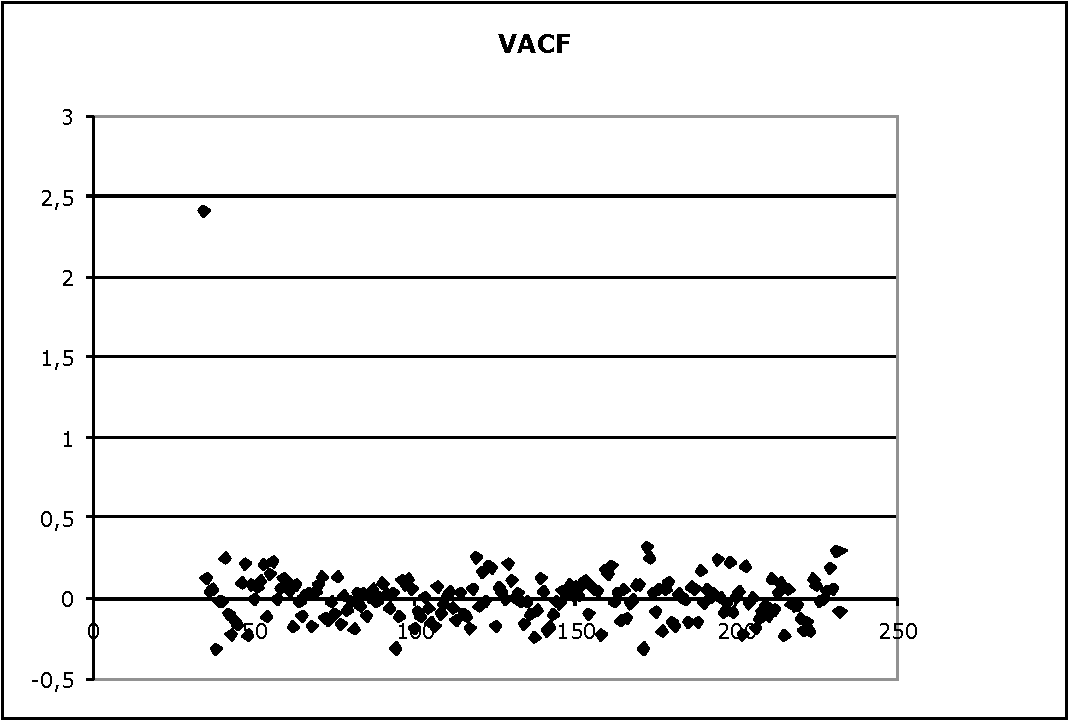
\includegraphics[width=10cm]{figures/vacf}
%\label{fig:vacf}
%\caption{The vacf.dat plot should be similar to this one}
%\end{center}
%\end{figure}
%
%\noindent We can see when time is larger than 50 the particles have already 'forgot' about their initial
%velocities. Sampling more in the time interval [0;50] will show the decay of VACF there.
%
%\newpage

\bibliographystyle{unsrt}
\bibliography{refs}
\end{document}
